
\documentclass[letterpaper,hide notes,xcolor={table,svgnames},pdftex,10pt]{beamer}
\def\showexamples{t}


%\usepackage[svgnames]{xcolor}

%% Demo talk
%\documentclass[letterpaper,notes=show]{beamer}

\usecolortheme{crane}
\setbeamertemplate{navigation symbols}{}

\usetheme{MyPittsburgh}
%\usetheme{Frankfurt}

%\usepackage{tipa}

\usepackage{hyperref}
\usepackage{graphicx,xspace}
\usepackage[normalem]{ulem}
\usepackage{multicol}
\usepackage{amsmath,amssymb,amsthm,graphicx,xspace}
\newcommand\SF[1]{$\bigstar$\footnote{SF: #1}}

\usepackage[default]{sourcesanspro}
\usepackage[T1]{fontenc}
\usepackage[scaled]{beramono}
\usepackage{tikzpagenodes}

\newcounter{tmpnumSlide}
\newcounter{tmpnumNote}


% old question code
%\newcommand\question[1]{{$\bigstar$ \small \onlySlide{2}{#1}}}
% \newcommand\nquestion[1]{\ifdefined \presentationonly \textcircled{?} \fi \note{\par{\Large \textbf{?}} #1}}
% \newcommand\nanswer[1]{\note{\par{\Large \textbf{A}} #1}}


 \newcommand\mnote[1]{%
   \addtocounter{tmpnumSlide}{1}
   \ifdefined\showcues {~\tiny\fbox{\arabic{tmpnumSlide}}}\fi
   \note{\setlength{\parskip}{1ex}\addtocounter{tmpnumNote}{1}\textbf{\Large \arabic{tmpnumNote}:} {#1\par}}}

\newcommand\mmnote[1]{\note{\setlength{\parskip}{1ex}#1\par}}

%\newcommand\mnote[2][]{\ifdefined\handoutwithnotes {~\tiny\fbox{#1}}\fi
% \note{\setlength{\parskip}{1ex}\textbf{\Large #1:} #2\par}}

%\newcommand\mnote[2][]{{\tiny\fbox{#1}} \note{\setlength{\parskip}{1ex}\textbf{\Large #1:} #2\par}}

\newcommand\mquestion[2]{{~\color{red}\fbox{?}}\note{\setlength{\parskip}{1ex}\par{\Large \textbf{?}} #1} \note{\setlength{\parskip}{1ex}\par{\Large \textbf{A}} #2\par}\ifdefined \presentationonly \pause \fi}

\newcommand\blackboard[1]{%
\ifdefined   \showblackboard
  {#1}
  \else {\begin{center} \fbox{\colorbox{blue!30}{%
         \begin{minipage}{.95\linewidth}%
           \hspace{\stretch{1}} Some space intentionally left blank; done at the blackboard.%
         \end{minipage}}}\end{center}}%
         \fi%
}



%\newcommand\q{\tikz \node[thick,color=black,shape=circle]{?};}
%\newcommand\q{\ifdefined \presentationonly \textcircled{?} \fi}

\usepackage{listings}
\lstset{basicstyle=\footnotesize\ttfamily,
	breaklines=true,
	aboveskip=15pt,
  	belowskip=15pt,
	frame=lines,
	numbers=left, basicstyle=\scriptsize, numberstyle=\tiny, stepnumber=0, numbersep=2pt
}

\usepackage{siunitx}
\newcommand\sius[1]{\num[group-separator = {,}]{#1}\si{\micro\second}}
\newcommand\sims[1]{\num[group-separator = {,}]{#1}\si{\milli\second}}
\newcommand\sins[1]{\num[group-separator = {,}]{#1}\si{\nano\second}}
\sisetup{group-separator = {,}, group-digits = true}

%% -------------------- tikz --------------------
\usepackage{tikz}
\usetikzlibrary{positioning}
\usetikzlibrary{arrows,backgrounds,automata,decorations.shapes,decorations.pathmorphing,decorations.markings,decorations.text,decorations.pathreplacing}

\tikzstyle{place}=[circle,draw=blue!50,fill=blue!20,thick, inner sep=0pt,minimum size=6mm]
\tikzstyle{transition}=[rectangle,draw=black!50,fill=black!20,thick, inner sep=0pt,minimum size=4mm]

\tikzstyle{block}=[rectangle,draw=black, thick, inner sep=5pt]
\tikzstyle{bullet}=[circle,draw=black, fill=black, thin, inner sep=2pt]

\tikzstyle{pre}=[<-,shorten <=1pt,>=stealth',semithick]
\tikzstyle{post}=[->,shorten >=1pt,>=stealth',semithick]
\tikzstyle{bi}=[<->,shorten >=1pt,shorten <=1pt, >=stealth',semithick]

\tikzstyle{mut}=[-,>=stealth',semithick]

\tikzstyle{treereset}=[dashed,->, shorten >=1pt,>=stealth',thin]

\usepackage{ifmtarg}
\usepackage{xifthen}
\makeatletter
% new counter to now which frame it is within the sequence
\newcounter{multiframecounter}
% initialize buffer for previously used frame title
\gdef\lastframetitle{\textit{undefined}}
% new environment for a multi-frame
\newenvironment{multiframe}[1][]{%
\ifthenelse{\isempty{#1}}{%
% if no frame title was set via optional parameter,
% only increase sequence counter by 1
\addtocounter{multiframecounter}{1}%
}{%
% new frame title has been provided, thus
% reset sequence counter to 1 and buffer frame title for later use
\setcounter{multiframecounter}{1}%
\gdef\lastframetitle{#1}%
}%
% start conventional frame environment and
% automatically set frame title followed by sequence counter
\begin{frame}%
\frametitle{\lastframetitle~{\normalfont(\arabic{multiframecounter})}}%
}{%
\end{frame}%
}
\makeatother

\makeatletter
\newdimen\tu@tmpa%
\newdimen\ydiffl%
\newdimen\xdiffl%
\newcommand\ydiff[2]{%
    \coordinate (tmpnamea) at (#1);%
    \coordinate (tmpnameb) at (#2);%
    \pgfextracty{\tu@tmpa}{\pgfpointanchor{tmpnamea}{center}}%
    \pgfextracty{\ydiffl}{\pgfpointanchor{tmpnameb}{center}}%
    \advance\ydiffl by -\tu@tmpa%
}
\newcommand\xdiff[2]{%
    \coordinate (tmpnamea) at (#1);%
    \coordinate (tmpnameb) at (#2);%
    \pgfextractx{\tu@tmpa}{\pgfpointanchor{tmpnamea}{center}}%
    \pgfextractx{\xdiffl}{\pgfpointanchor{tmpnameb}{center}}%
    \advance\xdiffl by -\tu@tmpa%
}
\makeatother
\newcommand{\copyrightbox}[3][r]{%
\begin{tikzpicture}%
\node[inner sep=0pt,minimum size=2em](ciimage){#2};
\usefont{OT1}{phv}{n}{n}\fontsize{4}{4}\selectfont
\ydiff{ciimage.south}{ciimage.north}
\xdiff{ciimage.west}{ciimage.east}
\ifthenelse{\equal{#1}{r}}{%
\node[inner sep=0pt,right=1ex of ciimage.south east,anchor=north west,rotate=90]%
{\raggedleft\color{black!50}\parbox{\the\ydiffl}{\raggedright{}#3}};%
}{%
\ifthenelse{\equal{#1}{l}}{%
\node[inner sep=0pt,right=1ex of ciimage.south west,anchor=south west,rotate=90]%
{\raggedleft\color{black!50}\parbox{\the\ydiffl}{\raggedright{}#3}};%
}{%
\node[inner sep=0pt,below=1ex of ciimage.south west,anchor=north west]%
{\raggedleft\color{black!50}\parbox{\the\xdiffl}{\raggedright{}#3}};%
}
}
\end{tikzpicture}
}


%% --------------------

%\usepackage[excludeor]{everyhook}
%\PushPreHook{par}{\setbox0=\lastbox\llap{MUH}}\box0}

%\vspace*{\stretch{1}

%\setbox0=\lastbox \llap{\textbullet\enskip}\box0}

\setlength{\parskip}{\fill}

\newcommand\noskips{\setlength{\parskip}{1ex}}
\newcommand\doskips{\setlength{\parskip}{\fill}}

\newcommand\xx{\par\vspace*{\stretch{1}}\par}
\newcommand\xxs{\par\vspace*{2ex}\par}
\newcommand\tuple[1]{\langle #1 \rangle}
\newcommand\code[1]{{\sf \footnotesize #1}}
\newcommand\ex[1]{\uline{Example:} \ifdefined \presentationonly \pause \fi
  \ifdefined\showexamples#1\xspace\else{\uline{\hspace*{2cm}}}\fi}

\newcommand\ceil[1]{\lceil #1 \rceil}


\AtBeginSection[]
{
   \begin{frame}
       \frametitle{Outline}
       \tableofcontents[currentsection]
   \end{frame}
}



\pgfdeclarelayer{edgelayer}
\pgfdeclarelayer{nodelayer}
\pgfsetlayers{edgelayer,nodelayer,main}

\tikzstyle{none}=[inner sep=0pt]
\tikzstyle{rn}=[circle,fill=Red,draw=Black,line width=0.8 pt]
\tikzstyle{gn}=[circle,fill=Lime,draw=Black,line width=0.8 pt]
\tikzstyle{yn}=[circle,fill=Yellow,draw=Black,line width=0.8 pt]
\tikzstyle{empty}=[circle,fill=White,draw=Black]
\tikzstyle{bw} = [rectangle, draw, fill=blue!20, 
    text width=4em, text centered, rounded corners, minimum height=2em]
    
    \newcommand{\CcNote}[1]{% longname
	This work is licensed under the \textit{Creative Commons #1 3.0 License}.%
}
\newcommand{\CcImageBy}[1]{%
	\includegraphics[scale=#1]{creative_commons/cc_by_30.pdf}%
}
\newcommand{\CcImageSa}[1]{%
	\includegraphics[scale=#1]{creative_commons/cc_sa_30.pdf}%
}
\newcommand{\CcImageNc}[1]{%
	\includegraphics[scale=#1]{creative_commons/cc_nc_30.pdf}%
}
\newcommand{\CcGroupBySa}[2]{% zoom, gap
	\CcImageBy{#1}\hspace*{#2}\CcImageNc{#1}\hspace*{#2}\CcImageSa{#1}%
}
\newcommand{\CcLongnameByNcSa}{Attribution-NonCommercial-ShareAlike}

\newenvironment{changemargin}[1]{% 
  \begin{list}{}{% 
    \setlength{\topsep}{0pt}% 
    \setlength{\leftmargin}{#1}% 
    \setlength{\rightmargin}{1em}
    \setlength{\listparindent}{\parindent}% 
    \setlength{\itemindent}{\parindent}% 
    \setlength{\parsep}{\parskip}% 
  }% 
  \item[]}{\end{list}} 




\title{Lecture 15 --- Memory Consistency}

\author{Patrick Lam \& Jeff Zarnett\\ \small \texttt{patrick.lam@uwaterloo.ca}, \texttt{jzarnett@uwaterloo.ca}}
\institute{Department of Electrical and Computer Engineering \\
  University of Waterloo}
\date{\today}


\begin{document}

\begin{frame}
  \titlepage

 \end{frame}
%%%%%%%%%%%%%%%%%%%%%%%%%%%%%%%%%%%%%%%%%%%%%%%%%%%%%%%%%%%%%%%%%%%%%%%%%%%%%%%%

\begin{frame}
  \frametitle{OpenMP Memory Model}

  \begin{changemargin}{1cm}
\large

  \begin{itemize}
    \item All threads share a single store called
      \structure{memory}.\\ ~~(may not actually represent RAM)\\[1em]
    \item Each thread has its own {\it temporary} view of memory.\\[1em]
    \item A thread's {\it temporary} view of memory\\ is not required to be
      consistent with memory.
  \end{itemize}~\\

  We'll talk more about memory models later.
  \end{changemargin}
  
\end{frame}
%%%%%%%%%%%%%%%%%%%%%%%%%%%%%%%%%%%%%%%%%%%%%%%%%%%%%%%%%%%%%%%%%%%%%%%%%%%%%%%%

%%%%%%%%%%%%%%%%%%%%%%%%%%%%%%%%%%%%%%%%%%%%%%%%%%%%%%%%%%%%%%%%%%%%%%%%%%%%%%%%
\begin{frame}[fragile]
  \frametitle{Preventing Simultaneous Execution?}

  \begin{lstlisting}[language=C,morekeywords={foreach,pragma,omp,parallel,single,nowait,task,untied,barrier,taskyield,mergeable,final,taskwait,critical}]
                    a = b = 0
/* thread 1 */                      /* thread 2 */

atomic(b = 1) // [1]                atomic(a = 1) // [3]
atomic(tmp = a) // [2]              atomic(tmp = b) // [4]
if (tmp == 0) then                  if (tmp == 0) then
    // protected section                // protected section
end if                              end if
  \end{lstlisting}


\large
 Does this code actually prevent simultaneous execution?

  
\end{frame}
%%%%%%%%%%%%%%%%%%%%%%%%%%%%%%%%%%%%%%%%%%%%%%%%%%%%%%%%%%%%%%%%%%%%%%%%%%%%%%%%

%%%%%%%%%%%%%%%%%%%%%%%%%%%%%%%%%%%%%%%%%%%%%%%%%%%%%%%%%%%%%%%%%%%%%%%%%%%%%%%%
\begin{frame}[fragile]
  \frametitle{Not seeing the problem...?}

  \begin{lstlisting}[language=C,morekeywords={foreach,pragma,omp,parallel,single,nowait,task,untied,barrier,taskyield,mergeable,final,taskwait,critical}]
                    a = b = 0
/* thread 1 */                      /* thread 2 */

atomic(b = 1) // [1]                atomic(a = 1) // [3]
atomic(tmp = a) // [2]              atomic(tmp = b) // [4]
if (tmp == 0) then                  if (tmp == 0) then
    // protected section                // protected section
end if                              end if
  \end{lstlisting}

  \begin{center}
  \begin{tabular}{r r r r | r r}
    \multicolumn{4}{c|}{Order} & t1 tmp & t2 tmp\\
    \hline
    1 & 2 & 3 & 4 & 0 & 1\\
    1 & 3 & 2 & 4 & 1 & 1\\
    1 & 3 & 4 & 2 & 1 & 1\\
    3 & 4 & 1 & 2 & 1 & 0\\
    3 & 1 & 2 & 4 & 1 & 1\\
    3 & 1 & 4 & 2 & 1 & 1\\
  \end{tabular}
  \end{center}

  

\large
    Looks like it (at least intuitively).


\end{frame}
%%%%%%%%%%%%%%%%%%%%%%%%%%%%%%%%%%%%%%%%%%%%%%%%%%%%%%%%%%%%%%%%%%%%%%%%%%%%%%%%

%%%%%%%%%%%%%%%%%%%%%%%%%%%%%%%%%%%%%%%%%%%%%%%%%%%%%%%%%%%%%%%%%%%%%%%%%%%%%%%%
\begin{frame}[fragile]
  \frametitle{The Memory Model Contains Gotchas}

  \begin{lstlisting}[language=C,morekeywords={foreach,pragma,omp,parallel,single,nowait,task,untied,barrier,taskyield,mergeable,final,taskwait,critical}]
                    a = b = 0
/* thread 1 */                      /* thread 2 */

atomic(b = 1) // [1]                atomic(a = 1) // [3]
atomic(tmp = a) // [2]              atomic(tmp = b) // [4]
if (tmp == 0) then                  if (tmp == 0) then
    // protected section                // protected section
end if                              end if
  \end{lstlisting}

  

\large
    Sorry! With OpenMP's memory model, no guarantees:\\
    the update from one thread may not be seen by the other.
    
\begin{center}
	
\includegraphics[width=0.4\textwidth]{images/oab.jpg}
\end{center}


\end{frame}
%%%%%%%%%%%%%%%%%%%%%%%%%%%%%%%%%%%%%%%%%%%%%%%%%%%%%%%%%%%%%%%%%%%%%%%%%%%%%%%%

%%%%%%%%%%%%%%%%%%%%%%%%%%%%%%%%%%%%%%%%%%%%%%%%%%%%%%%%%%%%%%%%%%%%%%%%%%%%%%%%
\begin{frame}[fragile]
  \frametitle{Flush Ensures Consistent Views of Memory}
\large
  \begin{center}
    {\tt \#pragma omp }{\bf flush} {\it[(list)]}
  \end{center}

    Makes the thread's temporary view of memory consistent with main
      memory.
    
    It enforces an order on memory operations of variables.
    
    The variables in the list are called the \alert{flush-set}.
    
    If no variables given, compiler determines them for you.
 
  
\end{frame}
%%%%%%%%%%%%%%%%%%%%%%%%%%%%%%%%%%%%%%%%%%%%%%%%%%%%%%%%%%%%%%%%%%%%%%%%%%%%%%%%

%%%%%%%%%%%%%%%%%%%%%%%%%%%%%%%%%%%%%%%%%%%%%%%%%%%%%%%%%%%%%%%%%%%%%%%%%%%%%%%%
\begin{frame}
  \frametitle{Flush: Before is Before, After is After}

  
\large
  Enforcing an order on the memory operations means:

  \begin{itemize}
    \item All read/write operations on the {\it flush-set} which happen
      before the {\bf flush} complete before the flush executes.
    \item All read/write operations on the {\it flush-set} which happen
      after the {\bf flush} complete after the flush executes.
    \item Flushes with overlapping {\it flush-sets} can not be reordered.
  \end{itemize}
  
\end{frame}
%%%%%%%%%%%%%%%%%%%%%%%%%%%%%%%%%%%%%%%%%%%%%%%%%%%%%%%%%%%%%%%%%%%%%%%%%%%%%%%%

%%%%%%%%%%%%%%%%%%%%%%%%%%%%%%%%%%%%%%%%%%%%%%%%%%%%%%%%%%%%%%%%%%%%%%%%%%%%%%%%
\begin{frame}
  \frametitle{Flush Correctness}
  
  To show a consistent value for a variable between two threads, 
  OpenMP must run statements in this order:

  \begin{enumerate}
    \item $t_1$ writes the value to $v$;
    \item $t_1$ flushes $v$; 
    \item $t_2$ flushes $v$ also;
    \item $t_2$ reads the consistent value from $v$.
  \end{enumerate}

\end{frame}
%%%%%%%%%%%%%%%%%%%%%%%%%%%%%%%%%%%%%%%%%%%%%%%%%%%%%%%%%%%%%%%%%%%%%%%%%%%%%%%%

%%%%%%%%%%%%%%%%%%%%%%%%%%%%%%%%%%%%%%%%%%%%%%%%%%%%%%%%%%%%%%%%%%%%%%%%%%%%%%%%
\begin{frame}[fragile]
  \frametitle{Take 2: Same Example, now improved with Flush}

  \begin{lstlisting}[language=C,morekeywords={foreach,pragma,omp,parallel,single,nowait,task,untied,barrier,taskyield,mergeable,final,taskwait,critical}]
                    a = b = 0
/* thread 1 */                      /* thread 2 */

atomic(b = 1)                       atomic(a = 1)
flush(b)                            flush(a)
flush(a)                            flush(b)
atomic(tmp = a)                     atomic(tmp = b)
if (tmp == 0) then                  if (tmp == 0) then
    // protected section                // protected section
end if                              end if
  \end{lstlisting}

\Large
Will this now prevent simultaneous access?

\end{frame}
%%%%%%%%%%%%%%%%%%%%%%%%%%%%%%%%%%%%%%%%%%%%%%%%%%%%%%%%%%%%%%%%%%%%%%%%%%%%%%%%

%%%%%%%%%%%%%%%%%%%%%%%%%%%%%%%%%%%%%%%%%%%%%%%%%%%%%%%%%%%%%%%%%%%%%%%%%%%%%%%%
\begin{frame}[fragile]
  \frametitle{No Luck Yet: Flush Fails}

  

  \begin{center}
    \alert{\LARGE No.}
  \end{center}

  \begin{itemize}
    \item The compiler can reorder the {\tt flush(b)} in thread~1 or
      {\tt flush(a)} in thread~2.

    \item If {\tt flush(b)} gets reordered to after the protected
      section, we will not get our intended operation.
  \end{itemize}
  
\end{frame}
%%%%%%%%%%%%%%%%%%%%%%%%%%%%%%%%%%%%%%%%%%%%%%%%%%%%%%%%%%%%%%%%%%%%%%%%%%%%%%%%

%%%%%%%%%%%%%%%%%%%%%%%%%%%%%%%%%%%%%%%%%%%%%%%%%%%%%%%%%%%%%%%%%%%%%%%%%%%%%%%%
\begin{frame}[fragile]
  \frametitle{Should you use flush?}

  
  \Large
  Probably not, but now you know what it does.
  

\end{frame}
%%%%%%%%%%%%%%%%%%%%%%%%%%%%%%%%%%%%%%%%%%%%%%%%%%%%%%%%%%%%%%%%%%%%%%%%%%%%%%%%


%%%%%%%%%%%%%%%%%%%%%%%%%%%%%%%%%%%%%%%%%%%%%%%%%%%%%%%%%%%%%%%%%%%%%%%%%%%%%%%%
\begin{frame}[fragile]
  \frametitle{Proper Use of Flush}

  \begin{lstlisting}[language=C,morekeywords={foreach,pragma,omp,parallel,single,nowait,task,untied,barrier,taskyield,mergeable,final,taskwait,critical}]
                    a = b = 0
/* thread 1 */                      /* thread 2 */

atomic(b = 1)                       atomic(a = 1)
flush(a, b)                         flush(a, b)
atomic(tmp = a)                     atomic(tmp = b)
if (tmp == 0) then                  if (tmp == 0) then
    // protected section                // protected section
end if                              end if
  \end{lstlisting}
\end{frame}
%%%%%%%%%%%%%%%%%%%%%%%%%%%%%%%%%%%%%%%%%%%%%%%%%%%%%%%%%%%%%%%%%%%%%%%%%%%%%%%%

%%%%%%%%%%%%%%%%%%%%%%%%%%%%%%%%%%%%%%%%%%%%%%%%%%%%%%%%%%%%%%%%%%%%%%%%%%%%%%%%
\begin{frame}
  \frametitle{OpenMP Directives Where Flush Is Implied}

\large
  \begin{itemize}
    \item {\tt omp barrier}
    \item at entry to, and exit from, {\bf omp critical};
    \item at exit from {\bf omp parallel}; 
    \item at exit from {\bf omp for};
    \item at exit from {\bf omp sections};
    \item at exit from {\bf omp single}.
  \end{itemize}

\end{frame}
%%%%%%%%%%%%%%%%%%%%%%%%%%%%%%%%%%%%%%%%%%%%%%%%%%%%%%%%%%%%%%%%%%%%%%%%%%%%%%%%

%%%%%%%%%%%%%%%%%%%%%%%%%%%%%%%%%%%%%%%%%%%%%%%%%%%%%%%%%%%%%%%%%%%%%%%%%%%%%%%%
\begin{frame} 
  \frametitle{OpenMP Directives Where Flush Isn't Implied}

\large
  \begin{itemize}
    \item at entry to {\bf for};
    \item at entry to, or exit from, {\bf master};
    \item at entry to {\bf sections}; 
    \item at entry to {\bf single};
    \item at exit from {\bf for}, {\bf single} or {\bf sections} with a {\bf nowait}
      \begin{itemize}
        \item {\bf nowait} removes implicit flush\\
 along with the implicit barrier
      \end{itemize}
  \end{itemize}

  This is not true for OpenMP versions before 2.5,\\
 so be careful.

\end{frame}
%%%%%%%%%%%%%%%%%%%%%%%%%%%%%%%%%%%%%%%%%%%%%%%%%%%%%%%%%%%%%%%%%%%%%%%%%%%%%%%%


%%%%%%%%%%%%%%%%%%%%%%%%%%%%%%%%%%%%%%%%%%%%%%%%%%%%%%%%%%%%%%%%%%%%%%%%%%%%%%%%
\begin{frame}
  \frametitle{Why Your Code is Slow}

  \large
  Want it to run faster? Avoid these pitfalls:\\
  \begin{enumerate}
    \item Unnecessary flush directives.
    \item Using critical sections or locks instead of atomic.
    \item Unnecessary concurrent-memory-writing protection:
      \begin{itemize}
        \item No need to protect local thread variables.
        \item No need to protect if only accessed in {\bf single} or
          {\bf master}.
      \end{itemize}
    \item Too much work in a critical section.
    \item Too many entries into critical sections.
  \end{enumerate}
  
\end{frame}
%%%%%%%%%%%%%%%%%%%%%%%%%%%%%%%%%%%%%%%%%%%%%%%%%%%%%%%%%%%%%%%%%%%%%%%%%%%%%%%%

%%%%%%%%%%%%%%%%%%%%%%%%%%%%%%%%%%%%%%%%%%%%%%%%%%%%%%%%%%%%%%%%%%%%%%%%%%%%%%%%
\begin{frame}[fragile]
  \frametitle{Example: Reducing Too Many Entries into Critical Sections}

  \large
  \begin{lstlisting}[language=C,morekeywords={foreach,pragma,omp,parallel,single,nowait,task,untied,barrier,taskyield,mergeable,final,taskwait,critical}]
#pragma omp parallel for
for (i = 0; i < N; ++i) { 
    #pragma omp critical
    {
        if (arr[i] > max) max = arr[i];
    } 
}
  \end{lstlisting}

would be better as:

  \begin{lstlisting}[language=C,morekeywords={foreach,pragma,omp,parallel,single,nowait,task,untied,barrier,taskyield,mergeable,final,taskwait,critical}]
#pragma omp parallel for
for (i = 0 ; i < N; ++i) { 
    #pragma omp flush(max)
    if (arr[i] > max) {
          #pragma omp critical
          {
                if (arr[i] > max) max = arr[i];
          }
    }
}
  \end{lstlisting}
  
\end{frame}
%%%%%%%%%%%%%%%%%%%%%%%%%%%%%%%%%%%%%%%%%%%%%%%%%%%%%%%%%%%%%%%%%%%%%%%%%%%%%%%%

%%%%%%%%%%%%%%%%%%%%%%%%%%%%%%%%%%%%%%%%%%%%%%%%%%%%%%%%%%%%%%%%%%%%%%%%%%%%%%%%
\begin{frame}
  \frametitle{OpenMP Wrap-up}

\Large
    Key points:\\
  \begin{itemize}
    \item How to use OpenMP {\bf tasks} to\\ \hspace*{2em} parallelize unstructured problems.
    \item How to use {\bf flush} correctly.
  \end{itemize}
  
\end{frame}
%%%%%%%%%%%%%%%%%%%%%%%%%%%%%%%%%%%%%%%%%%%%%%%%%%%%%%%%%%%%%%%%%%%%%%%%%%%%%%%%

\begin{frame}
  \frametitle{Memory Models}

  

  Sequential program: statements execute in order.\\

  Your expectation for concurrency: sequential consistency.

\begin{quote}
``... the result of any execution is the same as if the operations of all the processors were executed in some sequential order, and the operations of each individual processor appear in this sequence in the order specified by its program.'' --- Leslie Lamport
\end{quote}
  In brief:
  \begin{enumerate}
  \item for each thread: in-order execution;
  \item interleave the threads' executions.
  \end{enumerate}~\\

  No one has it: too expensive; recall the worked example for {\bf flush} last time.

\end{frame}



\begin{frame}
  \frametitle{Memory Models: Sequential Consistency}

  
    Another view of sequential consistency:

    \begin{itemize}
      \item each thread induces an \emph{execution trace}.
      \item always: program has executed some prefix of each thread's
        trace.
    \end{itemize}
  
\end{frame}

\begin{frame}
\frametitle{The Blind Men and Elephant}

\begin{center}
	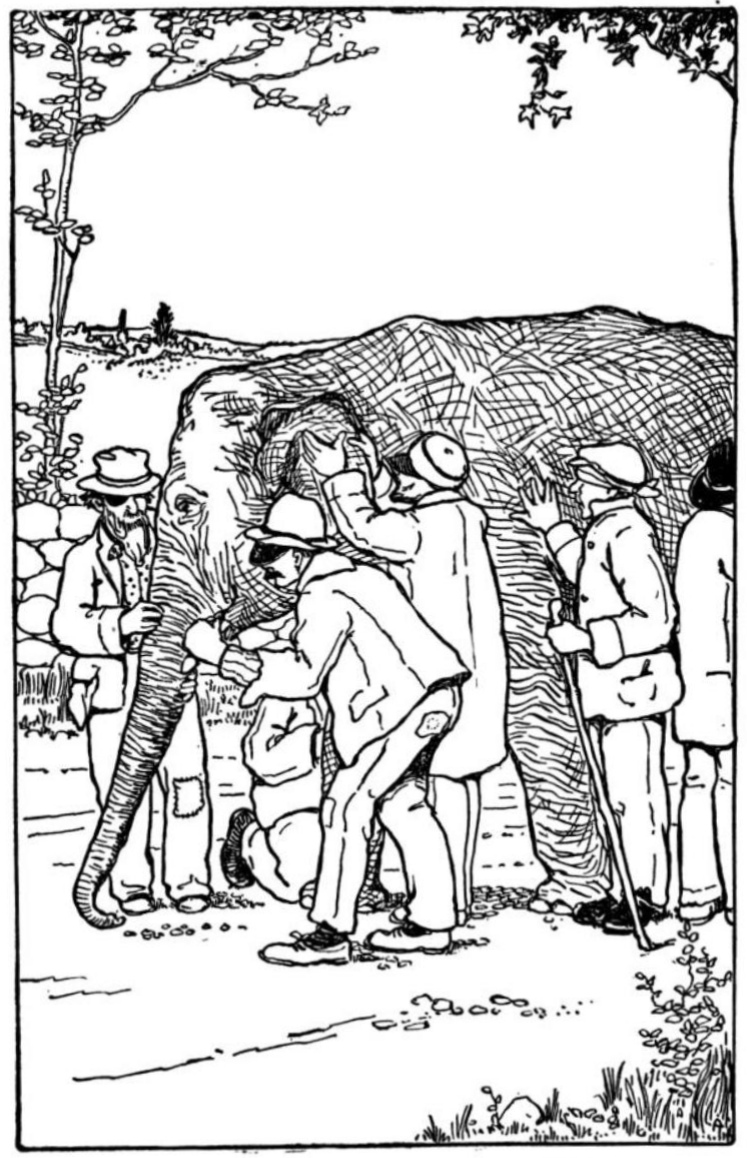
\includegraphics[width=0.4\textwidth]{images/Blind_men_and_elephant.jpg}
\end{center}

But unfortunately, threads have their own view of the world.

\end{frame}

\begin{frame}
  \frametitle{Reordering}

  
     Compilers and processors may reorder non-interfering memory
     operations.

      \[ T1: x = 1; r1 = y; \]

     If two statements are independent:
     \begin{itemize}
        \item OK to execute them in either order.
        \item (equivalently: publish their results to other threads).
     \end{itemize}

     Reordering is a major compiler tactic to produce speedup.
  
\end{frame}

%%%%%%%%%%%%%%%%%%%%%%%%%%%%%%%%%%%%%%%%%%%%%%%%%%%%%%%%%%%%%%%%%%%%%%%%%%%%%%%%

%%%%%%%%%%%%%%%%%%%%%%%%%%%%%%%%%%%%%%%%%%%%%%%%%%%%%%%%%%%%%%%%%%%%%%%%%%%%%%%%
\begin{frame}
  \frametitle{Memory Consistency Models}

  
    Sequential consistency:
      \begin{itemize}
        \item No reordering of loads/stores.
      \end{itemize}
    Sequential consistency for datarace-free programs:
      \begin{itemize}
        \item If your program
  has no data races, then sequential consistency.
      \end{itemize}
    Relaxed consistency (only some types of reorderings):
      \begin{itemize}
        \item Loads can be reordered after loads/stores; and
        \item Stores can be reordered after loads/stores.
      \end{itemize}
    Weak consistency:
      \begin{itemize}
        \item Any reordering is possible.
      \end{itemize}

  Still, {\bf reorderings} only allowed if they look safe in current context
  (i.e. independent; different memory addresses).
  
\end{frame}
%%%%%%%%%%%%%%%%%%%%%%%%%%%%%%%%%%%%%%%%%%%%%%%%%%%%%%%%%%%%%%%%%%%%%%%%%%%%%%%%

%%%%%%%%%%%%%%%%%%%%%%%%%%%%%%%%%%%%%%%%%%%%%%%%%%%%%%%%%%%%%%%%%%%%%%%%%%%%%%%%
\begin{frame}[fragile]
  \frametitle{2011 Final Exam Question}

  
  \begin{lstlisting}[language=C]
                       x = y = 0

/* thread 1 */                    /* thread 2 */
x = 1;                            y = x;
r1 = y;                           r2 = x;
  \end{lstlisting}

  Assume architecture not sequentially consistent\\ \hspace*{3em} (weak~consistency).

  Show me all possible (intermediate and final) memory values and how they arise.
  
\end{frame}
%%%%%%%%%%%%%%%%%%%%%%%%%%%%%%%%%%%%%%%%%%%%%%%%%%%%%%%%%%%%%%%%%%%%%%%%%%%%%%%%

%%%%%%%%%%%%%%%%%%%%%%%%%%%%%%%%%%%%%%%%%%%%%%%%%%%%%%%%%%%%%%%%%%%%%%%%%%%%%%%%
\begin{frame}[fragile]
  \frametitle{2011 Final Exam Question: Solution}

  
    Must include every permutation of lines (since they can be in
      any order);\\
    then iterate over all the values.\\[1em]

    Probably too long, but shows how memory reorderings
      complicate things.
  
\end{frame}
%%%%%%%%%%%%%%%%%%%%%%%%%%%%%%%%%%%%%%%%%%%%%%%%%%%%%%%%%%%%%%%%%%%%%%%%%%%%%%%%

%%%%%%%%%%%%%%%%%%%%%%%%%%%%%%%%%%%%%%%%%%%%%%%%%%%%%%%%%%%%%%%%%%%%%%%%%%%%%%%%
\begin{frame}[fragile]
  \frametitle{The Compiler Reorders Memory Accesses}

  
  When it can prove safety, the {\bf compiler} may reorder instructions (not just the hardware).\\[1em]

  {\bf Example:} want thread 1 to print value set in thread 2.

  \begin{lstlisting}[language=C]
                            f = 0

/* thread 1 */                          /* thread 2 */
while (f == 0) /* spin */;              x = 42;
printf("%d", x);                        f = 1;
  \end{lstlisting}

  \begin{itemize}
    \item If thread 2 reorders its instructions, will we get our intended
      result?\\[1em]
    \only<2-> \alert{~~~~~No.}
  \end{itemize}
  
\end{frame}
%%%%%%%%%%%%%%%%%%%%%%%%%%%%%%%%%%%%%%%%%%%%%%%%%%%%%%%%%%%%%%%%%%%%%%%%%%%%%%%%


\begin{frame}
\frametitle{KEEP OUT}

\begin{center}
	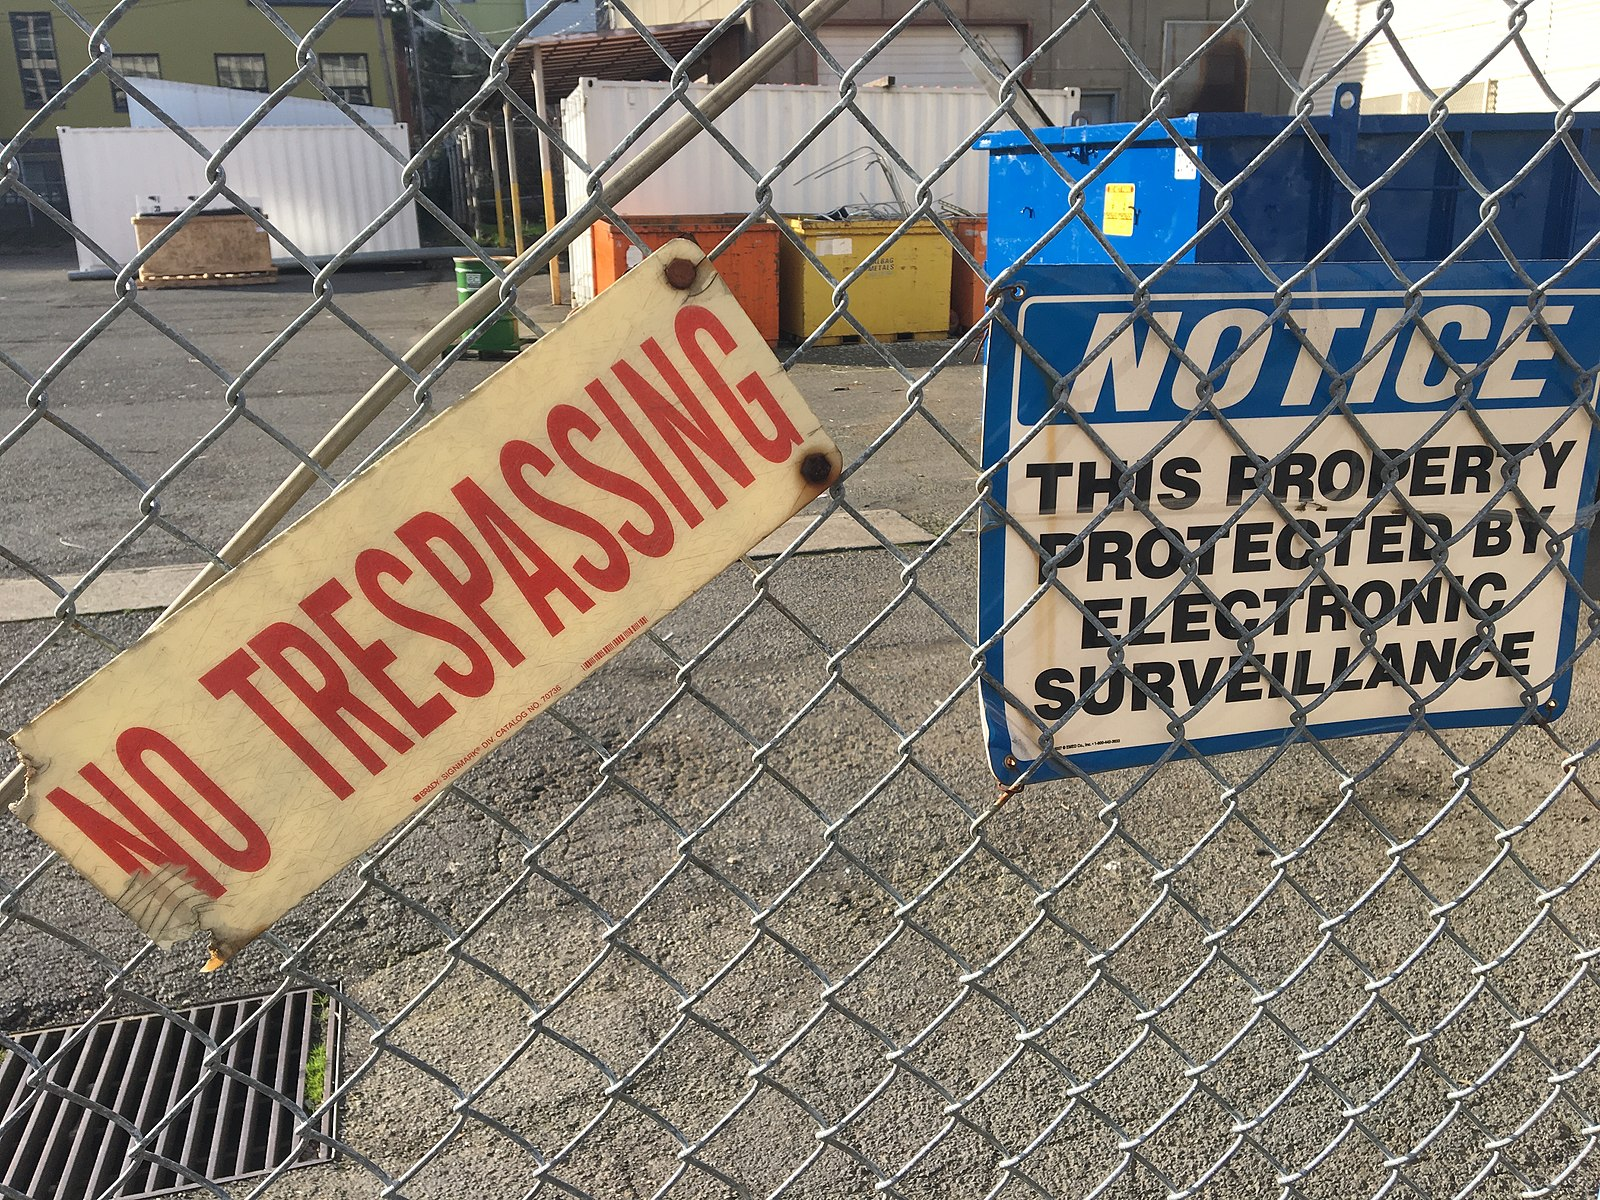
\includegraphics[width=0.7\textwidth]{images/No_trespassing.jpg}
\end{center}
\hfill Image Credit: MB298


\end{frame}



%%%%%%%%%%%%%%%%%%%%%%%%%%%%%%%%%%%%%%%%%%%%%%%%%%%%%%%%%%%%%%%%%%%%%%%%%%%%%%%%
\begin{frame}[fragile]
  \frametitle{Preventing Memory Reordering}

  
     A {\bf memory fence} prevents memory operations from crossing the
      fence (also known as a {\bf memory barrier}).

  \begin{lstlisting}[language=C]
                         f = 0

/* thread 1 */                     /* thread 2 */
while (f == 0) /* spin */;         x = 42;
// memory fence                    // memory fence
printf("%d", x);                   f = 1;
  \end{lstlisting}

  \begin{itemize}
    \item Now prevents reordering; get expected result.
  \end{itemize}
  

\end{frame}
%%%%%%%%%%%%%%%%%%%%%%%%%%%%%%%%%%%%%%%%%%%%%%%%%%%%%%%%%%%%%%%%%%%%%%%%%%%%%%%%

%%%%%%%%%%%%%%%%%%%%%%%%%%%%%%%%%%%%%%%%%%%%%%%%%%%%%%%%%%%%%%%%%%%%%%%%%%%%%%%%
\begin{frame}[fragile]
  \frametitle{Preventing Memory Reordering in Programs}

  
     Step 1: Don't use volatile on C/C++ variables~\footnote{\tiny \url{http://stackoverflow.com/questions/78172/using-c-pthreads-do-shared-variables-need-to-be-volatile}.}.
     
     Syntax depends on the compiler.

\begin{itemize}
  \item Microsoft Visual Studio C++ Compiler:
  \begin{lstlisting}[language=C]
_ReadWriteBarrier()
  \end{lstlisting}
  \item Intel Compiler:
  \begin{lstlisting}[language=C]
    __memory_barrier()
  \end{lstlisting}
  \item GNU Compiler:
  \begin{lstlisting}[language=C]
__asm__ __volatile__ ("" ::: "memory");
  \end{lstlisting}
\end{itemize}

  The compiler also shouldn't reorder across e.g. pthreads mutex calls.
  
\end{frame}
%%%%%%%%%%%%%%%%%%%%%%%%%%%%%%%%%%%%%%%%%%%%%%%%%%%%%%%%%%%%%%%%%%%%%%%%%%%%%%%%

%%%%%%%%%%%%%%%%%%%%%%%%%%%%%%%%%%%%%%%%%%%%%%%%%%%%%%%%%%%%%%%%%%%%%%%%%%%%%%%%
\begin{frame}[fragile]
  \frametitle{Aside: {\tt gcc} Inline Assembly}

  

  Just as an aside, here's {\tt gcc}'s inline assembly format

  \begin{lstlisting}[language=C]
__asm__ ( assembler template 
       : output operands                  /* optional */
       : input operands                   /* optional */
       : list of clobbered registers      /* optional */
       );
  \end{lstlisting}
  \vfill
  Last slide used {\bf \_\_volatile\_\_} with  \_\_asm\_\_. This isn't the same as the normal C volatile. It means:

  \begin{itemize}
    \item The compiler may not reorder this assembly code\\ and put it somewhere
      else in the program.
  \end{itemize}
  

\end{frame}
%%%%%%%%%%%%%%%%%%%%%%%%%%%%%%%%%%%%%%%%%%%%%%%%%%%%%%%%%%%%%%%%%%%%%%%%%%%%%%%%

%%%%%%%%%%%%%%%%%%%%%%%%%%%%%%%%%%%%%%%%%%%%%%%%%%%%%%%%%%%%%%%%%%%%%%%%%%%%%%%%
\begin{frame}
  \frametitle{Memory Fences: Preventing HW Memory Reordering}


Memory barrier: no access after the barrier becomes visible to the
system (i.e. takes effect) until after all accesses before the barrier
become visible.\\[1em]

  {\bf Note:} these are all x86 {\tt asm} instructions.\\[1em]
  {\tt mfence}:
  \begin{itemize}
    \item All loads and stores before the fence finish before any more loads or stores execute.
  \end{itemize}
  {\tt sfence}:
  \begin{itemize}
    \item All stores before the fence finish before any more stores execute.
  \end{itemize}
  {\tt lfence}:
  \begin{itemize}
    \item All loads before the fence finish before any more loads execute.
  \end{itemize}
  
\end{frame}
%%%%%%%%%%%%%%%%%%%%%%%%%%%%%%%%%%%%%%%%%%%%%%%%%%%%%%%%%%%%%%%%%%%%%%%%%%%%%%%%

%%%%%%%%%%%%%%%%%%%%%%%%%%%%%%%%%%%%%%%%%%%%%%%%%%%%%%%%%%%%%%%%%%%%%%%%%%%%%%%%
\begin{frame}[fragile]
  \frametitle{Preventing Hardware Memory Reordering (Option 2)}

  
  Some compilers also support preventing hardware reordering:

\begin{itemize}
  \item Microsoft Visual Studio C++ Compiler:
  \begin{lstlisting}[language=C]
MemoryBarrier();
  \end{lstlisting}

  \item Solaris Studio (Oracle) Compiler:
  \begin{lstlisting}[language=C]
__machine_r_barrier();
__machine_w_barrier();
__machine_rw_barrier();
  \end{lstlisting}

  \item GNU Compiler:
  \begin{lstlisting}[language=C]
__sync_synchronize();
  \end{lstlisting}
\end{itemize}
  
\end{frame}
%%%%%%%%%%%%%%%%%%%%%%%%%%%%%%%%%%%%%%%%%%%%%%%%%%%%%%%%%%%%%%%%%%%%%%%%%%%%%%%%

  
%%%%%%%%%%%%%%%%%%%%%%%%%%%%%%%%%%%%%%%%%%%%%%%%%%%%%%%%%%%%%%%%%%%%%%%%%%%%%%%%
\begin{frame}
  \frametitle{Memory Barriers and OpenMP}

  
    Fortunately, an OpenMP {\bf flush} (or, better yet, mutexes) also preserve the order of variable accesses.\\[1em]
    Stops reordering from both the compiler and hardware.\\[1em]
    For GNU, flush is implemented as
      {\tt \_\_sync\_synchronize();}\\[1em]

  {\bf Note:} proper use of memory fences makes {\tt volatile} not very
  useful (again, {\tt volatile} is not meant to help with threading, and will
  have a different behaviour for threading on different compilers/hardware).
  
\end{frame}
%%%%%%%%%%%%%%%%%%%%%%%%%%%%%%%%%%%%%%%%%%%%%%%%%%%%%%%%%%%%%%%%%%%%%%%%%%%%%%%%


\begin{frame}
\frametitle{Atomic Operations}

\begin{center}
	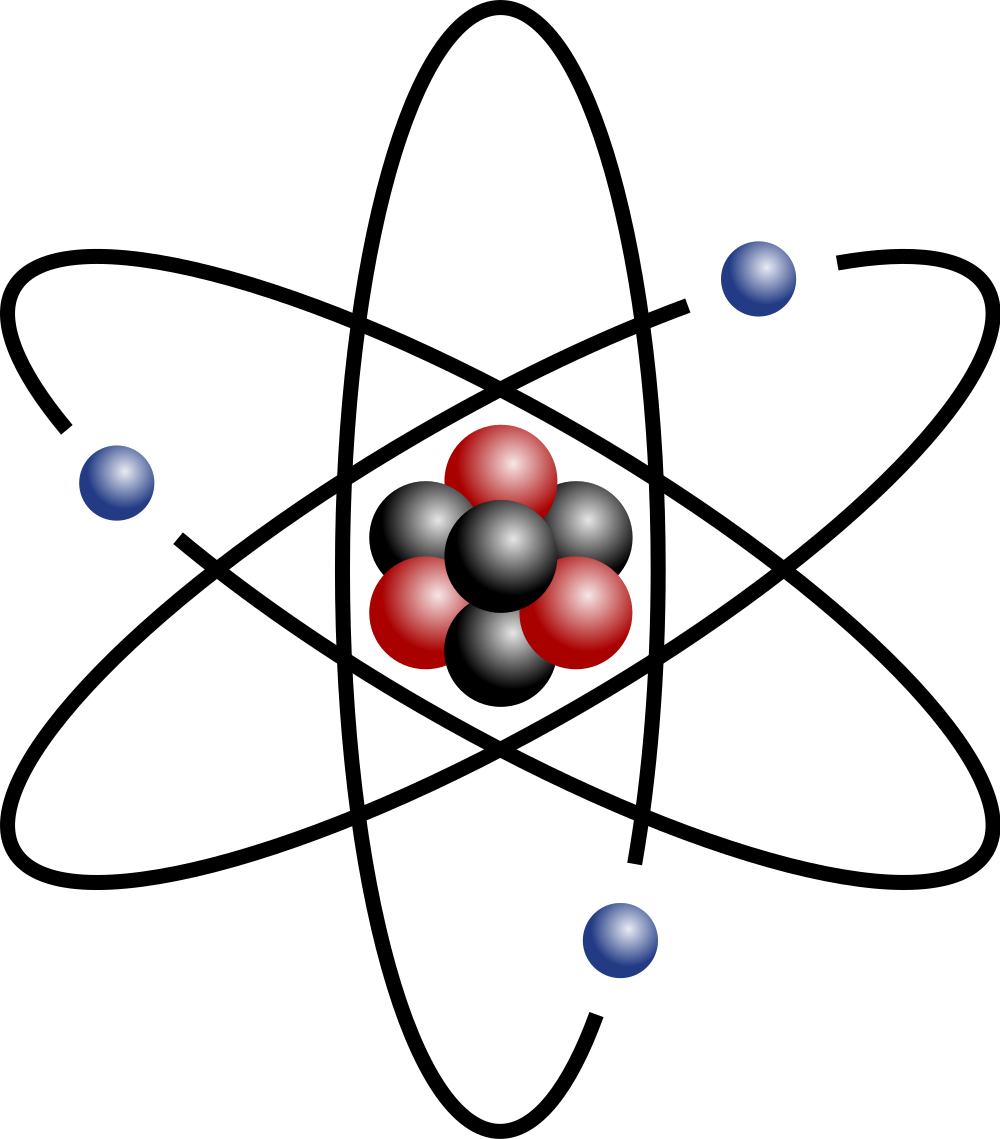
\includegraphics[width=0.4\textwidth]{images/atomic.png}
\end{center}

\url{https://commons.wikimedia.org/w/index.php?curid=1675352}

\end{frame}


%%%%%%%%%%%%%%%%%%%%%%%%%%%%%%%%%%%%%%%%%%%%%%%%%%%%%%%%%%%%%%%%%%%%%%%%%%%%%%%%
\begin{frame}
  \frametitle{Atomic Operations}

  

 We saw the {\bf atomic} directive in OpenMP, plus C++11 atomics.

 Most OpenMP atomic expressions map to atomic hardware instructions.

 Other atomic instructions exist.
  

\end{frame}
%%%%%%%%%%%%%%%%%%%%%%%%%%%%%%%%%%%%%%%%%%%%%%%%%%%%%%%%%%%%%%%%%%%%%%%%%%%%%%%%

%%%%%%%%%%%%%%%%%%%%%%%%%%%%%%%%%%%%%%%%%%%%%%%%%%%%%%%%%%%%%%%%%%%%%%%%%%%%%%%%
\begin{frame}[fragile]
  \frametitle{Compare and Swap}

  
  Also called {\bf compare and exchange} ({\tt cmpxchg} instruction).

  \begin{lstlisting}[language=C]
int compare_and_swap (int* reg, int oldval, int newval) {
  int old_reg_val = *reg;
  if (old_reg_val == oldval) 
     *reg = newval;
  return old_reg_val;
}
  \end{lstlisting}

  \begin{itemize}
    \item Afterwards, you can check if it returned {\tt oldval}.
    \item If it did, you know you changed it.
  \end{itemize}
  
\end{frame}
%%%%%%%%%%%%%%%%%%%%%%%%%%%%%%%%%%%%%%%%%%%%%%%%%%%%%%%%%%%%%%%%%%%%%%%%%%%%%%%%

%%%%%%%%%%%%%%%%%%%%%%%%%%%%%%%%%%%%%%%%%%%%%%%%%%%%%%%%%%%%%%%%%%%%%%%%%%%%%%%%
\begin{frame}[fragile]
  \frametitle{Implementing a Spinlock}

  
  Use compare-and-swap to implement spinlock:
  \begin{lstlisting}[language=C]
void spinlock_init(int* lock) { *lock = 0; }

void spinlock_lock(int* lock) {
    while(compare_and_swap(lock, 0, 1) != 0) {}
    __asm__ ("mfence");
}

void spinlock_unlock(int* lock) {
    __asm__ ("mfence");
    *lock = 0;  
}
  \end{lstlisting}
  You'll see {\bf cmpxchg} quite frequently in the Linux kernel code.
  
\end{frame}
%%%%%%%%%%%%%%%%%%%%%%%%%%%%%%%%%%%%%%%%%%%%%%%%%%%%%%%%%%%%%%%%%%%%%%%%%%%%%%%%

%%%%%%%%%%%%%%%%%%%%%%%%%%%%%%%%%%%%%%%%%%%%%%%%%%%%%%%%%%%%%%%%%%%%%%%%%%%%%%%%
\begin{frame}[fragile]
  \frametitle{ABA Problem}

  
    Sometimes you'll read a location twice.\\[1em]

    If the value is the same, nothing has changed, right?

    \pause

    \alert{No.} This is an {\bf ABA problem}.\\[1em]

    You can combat this by ``tagging'': modify value with nonce upon each write.\\[1em]

    Can keep value separately from nonce; double compare and swap atomically swaps both value and nonce.\\[2em]


  
\end{frame}
%%%%%%%%%%%%%%%%%%%%%%%%%%%%%%%%%%%%%%%%%%%%%%%%%%%%%%%%%%%%%%%%%%%%%%%%%%%%%%%%


\begin{frame}
\frametitle{Waterloo...}

\begin{center}
	
\includegraphics[width=0.7\textwidth]{images/abba.jpeg}
\end{center}

The ABA problem is not any sort of acronym nor a reference to this: \url{https://www.youtube.com/watch?v=Sj_9CiNkkn4}


\end{frame}



\begin{frame}
\frametitle{ABA}

It's a value that is A, then changed to B, then changed back to A. 

The ABA problem is a big mess for the designer of lock-free Compare-And-Swap routines. 

\begin{enumerate}
	\item $P_{1}$ reads $A_{i}$ from location $L_{i}$.
	\item $P_{k}$ interrupts $P_{1}$; $P_{k}$ stores the value $B$ into $L_{i}$.
	\item $P_{j}$ stores the value $A_{i}$ into $L_{i}$.
	\item $P_{1}$ resumes; it executes a false positive CAS.
\end{enumerate} 


\end{frame}



\begin{frame}
\frametitle{False Positive}

It's a ``false positive'' because $P_{1}$'s compare-and-swap operation succeeds even though the value at $L_{i}$ has been modified in the meantime. 

If this doesn't seem like a bad thing, consider this. 

If you have a data structure that will be accessed by multiple threads, you might be controlling access to it by the compare-and-swap routine. 

What should happen is the algorithm should keep trying until the data structure in question has not been modified by any other thread in the meantime. 

But with a false positive we get the impression that things didn't change, even though they really did.

\end{frame}



\begin{frame}
\frametitle{Napoleon was defeated...}

You can combat this by ``tagging'': modify value with nonce upon each
write.  

You can also keep the value separately from the nonce; double
compare and swap atomically swaps both value and nonce.

Another example of this: Java \texttt{ConcurrentModificationException} is detected by checking the modification count of a collection.

\end{frame}


\end{document}

